\section{Lexikální analýza}

Při tvorbě lexikálního analyzátoru bylo nejprve nutné převést jenotlivé lexémy (popsané regularními výrazy) na deterministický konečný automat. Dále jsme určili množinu speciálních identifikátorů - množinu klíčových slov. Automat obsahuje rozšíření o možnost blokových komentářů. Celkové schéma automatu popisuje vložený obrázek.

\begin{center}
 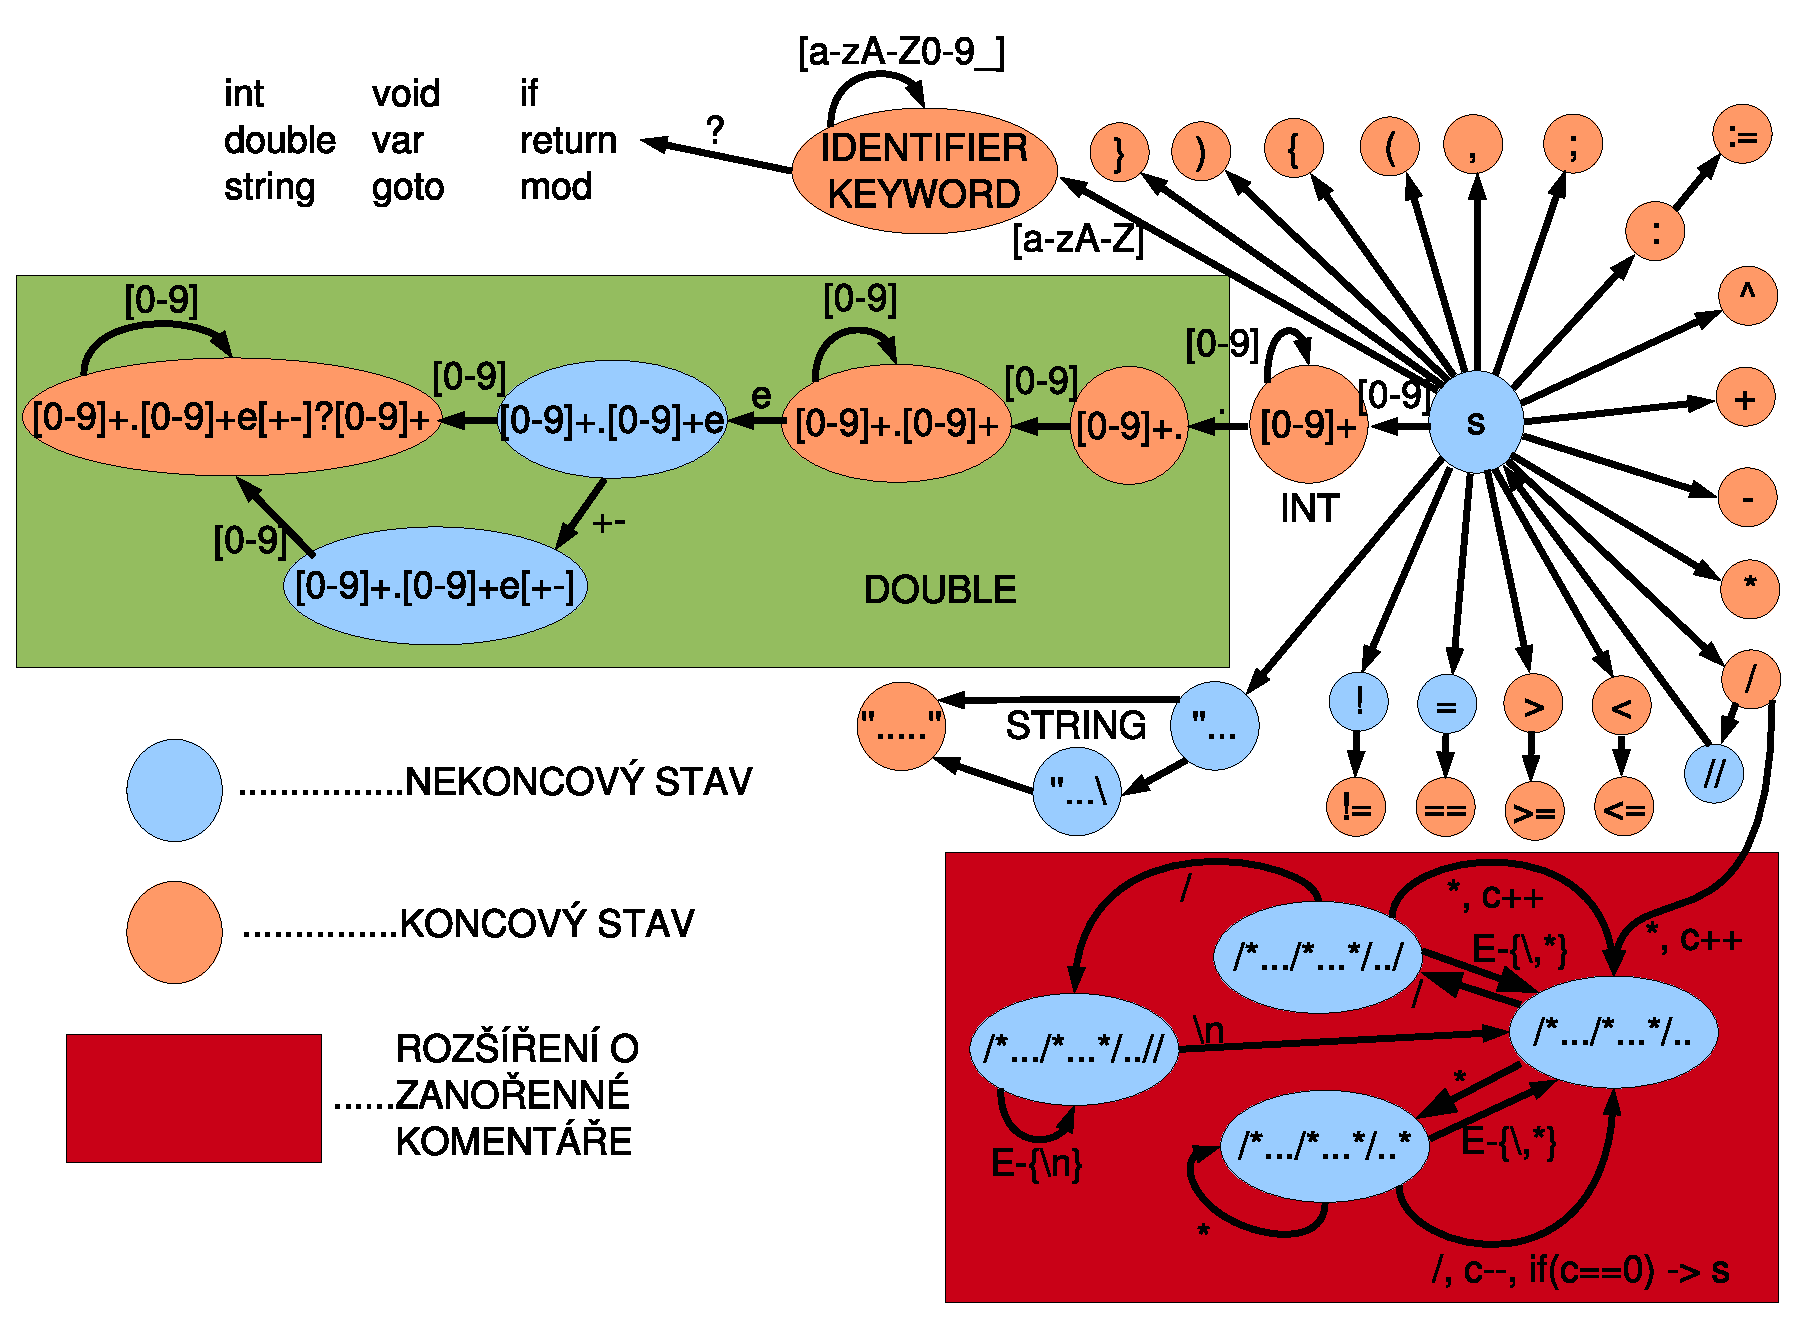
\includegraphics[scale=0.5]{include/scanner.eps}
\end{center}

Automat byl implementován nekonečným cyklem. Pokus o vyskočení z cyklu v nekoncovém stavu znamená chybný lexém a konec programu. Automat je schopen načítat lexémy libovolné délky, kontroluje přetečení při konverzi a zaznamenává pozici v načítaném souboru.
